\section{Differential Privacy for Count Queries }\label{sec3}
In this section, we introduce the concept of count queries within the framework of differential privacy,  a topic that has garnered substantial research attention.

\subsection{Essential Information of Count Queries}
For a time series $S$ comprising categorical values with length $t$ ($t$ can be $\infty$), a count query can be formally expressed as follow:
\begin{equation}\nonumber
	\mathrm{F}_{\mathrm{cnt}}(v, S)=\sum_{i=1}^{t}\mathbf{1}_v(x_i),
\end{equation}
where $\mathbf{1}_v(x_i)$ denotes the indicator function, defined below:
\begin{equation}\nonumber
	\mathbf{1}_v(x_i) :=
	\begin{cases} 
		1 & \text{if } x_i=v, \\
		0 & \text{if } x_i \ne v.
	\end{cases}
\end{equation}
Count queries are fundamental in the context of differential privacy, as they form the basis for other tasks, such as frequency and histogram estimations. 
 Compared with other scenarios, applying count queries to time series presents unique challenges. Time series arrives as a continuous stream, necessitating the injection of a larger amount of noise to provide the desired privacy guarantees due to continuous release of query results. 
 


\subsection{Core Techniques in Count Queries}
For continuously releasing a finite time series, a naive approach is to release each element with the entire privacy budget $\epsilon$~\cite{chan2011private}. However, such a method would introduce substantial additive noise, leading to low utility with an error bound of $O(\frac{\sqrt{T}}{\epsilon})$. 
Dwork et al.~\cite{dwork2010differential} proposed the first work to handle binary time series under event-level CDP with a logarithm error bound. However, this mechanism is limited to time series with finite length $T$. Subsequently, Chan et al.~\cite{chan2011private} improved the mechanism to support the release of infinite binary time series. Both of these works employ a tree-based method to enhance utility. The binary tree mechanism~\cite{chan2011private}, illustrated in Fig.~\ref{tree_mechanism}, ensures that each release influences at most one node at each level for finite time series. Consequently, each node only needs to add noise corresponding to the privacy budget $\frac{\epsilon}{(\log T+1)}$. To guarantee a logarithm error bound for infinite time series~\cite{chan2011private, dong2023continual}, more binary trees will be construed. Since the update of one element only influences one tree, each tree will be allocated an entire privacy budget. More details can be referred to Fig.~\ref{tree_mechanism}.

\begin{figure}[h]
	\centering
	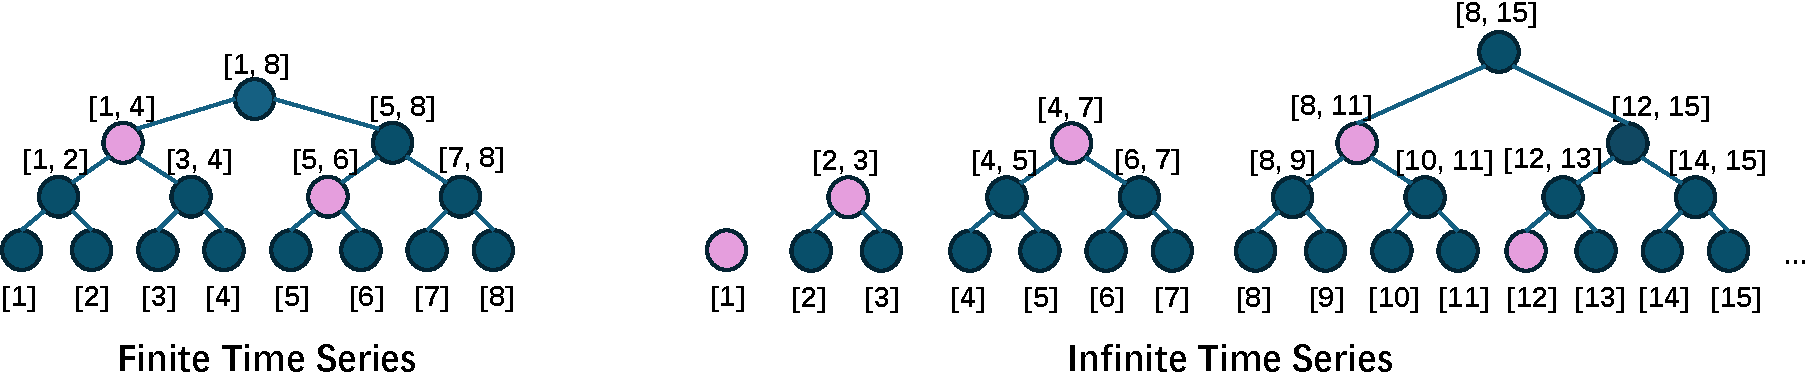
\includegraphics[width=0.8\textwidth]{submissions/submission4/figs/03-count/tree_mechanism-crop.pdf}
%	\caption{For finite time series $[1, 8]$ (i.e., $T=8$), the count query result for the range $[1, 6]$ is specified as $\mathrm{\hat{F}}_{\mathrm{cnt}}(1, [1, 6])=\mathrm{F}_{\mathrm{cnt}}(1, [1, 4])+\mathrm{F}_{\mathrm{cnt}}(1, [5, 6])+2Lap(\frac{\log T+1}
%	{\epsilon})$, where $Lap(b)$ is the Laplace distribution with zero mean. For an infinite time series at timestamp $t$, the mechanism first finds the timestamp $T=2^{\lfloor\log t\rfloor}$ and obtains $\mathrm{\hat{F}}_{\mathrm{cnt}}(1, [1, T])=\mathrm{F}_{\mathrm{cnt}}(1, [1, T])+Lap(\frac{2}{\epsilon})$. Additionally, elements exceeding the power of two (i.e., $[5, 6]$ with length $T'=2$) are processed as a finite time series. Namely, $\mathrm{\hat{F}}_{\mathrm{cnt}}(1, [1, 6])=\mathrm{F}_{\mathrm{cnt}}(1, [1, 4])+Lap(\frac{2}
%	{\epsilon})+\mathrm{F}_{\mathrm{cnt}}(1, [5, 6])+Lap(\frac{\log T'+1}
%	{\epsilon})$.}
 	\caption{Here is an illustration of binary tree mechanism for time series count query under event-level CDP. For finite time series $[1, 8]$ (i.e., $T=8$), the count query result for the range $[1, 6]$ is specified as $\mathrm{\hat{F}}_{\mathrm{cnt}}(v, [1, 6])=\mathrm{F}_{\mathrm{cnt}}(v, [1, 4])+\mathrm{F}_{\mathrm{cnt}}(v, [5, 6])+2Lap(\frac{\log T+1}{\epsilon})$, where $Lap(\cdot)$ is drawn from the Laplace distribution with zero mean. For an infinite time series, multiple binary trees will be constructed. Since a change in any single element only influences one tree, each tree will be allocated an entire privacy budget. The overall privacy budget consumption of the mechanism is $\epsilon$, which can be calculated using parallel composition~\cite{li2017differential}. For example, $\mathrm{\hat{F}}_{\mathrm{cnt}}(v, [1, 12])=\mathrm{\hat{F}}_{\mathrm{cnt}}(v, [1, 1])+\mathrm{\hat{F}}_{\mathrm{cnt}}(v, [2, 3])+\mathrm{\hat{F}}_{\mathrm{cnt}}(v, [4, 7])+\mathrm{\hat{F}}_{\mathrm{cnt}}(v, [8, 11])+\mathrm{\hat{F}}_{\mathrm{cnt}}(v, [12, 12])$.}
	\label{tree_mechanism}
\end{figure}


In addition to the tree-based structure, another approach to handle time series under differential privacy is based on the matrix mechanism~\cite{li2015matrix, henzinger2023almost}.
 Without privacy concerns, a count query $\mathcal{M}$ for binary time series $x$ with length $n$ can be specified as 
\begin{equation}
	\mathcal{M}(x) = Mx= \begin{bmatrix}\nonumber
		1 & 0 & 0 & \cdots  \\
		1 & 1 & 0 & \cdots \\
		1 & 1 & 1 & \cdots \\
		\vdots& \vdots & \vdots & \ddots
	\end{bmatrix} x = \begin{bmatrix}
	x_1\\
	x_1+x_2 \\
	\vdots \\
	\sum_{1}^{n} x_i
\end{bmatrix}.
\end{equation}
Based on this formulation, the matrix mechanism is employed to release data streams under $(\epsilon, \delta)$-DP for further error reduction. Given a workload matrix $M$, the strategy matrix $R$ and reconstruction matrix $L$ are first constructed, denoted as $M=LR$. The strategy matrix $R$ is utilized to pre-process the input $x$. After adding a Gaussian noise vector $z$ to the processed term $Rx$, a post-processing step $L$ is applied. In summary, for an input time series $x\in \mathbb{R}^n$, the matrix mechanism is denoted as 
\begin{equation}\nonumber
	\mathcal{M}_{L, R}(x)=L(Rx+z),
\end{equation}
where $z\sim N(0, \lVert R \rVert^2_{1\to 2}C^2_{\epsilon, \delta}\textbf{I})$ to ensure $(\epsilon, \delta)$-DP, $\lVert R \rVert^2_{1\to 2}$ is the maximum of the 2-norm of the columns of the strategy matrix $R$. The additive mean squared error $\mathrm{err}_{\ell^2_2}$ of the matrix mechanism is 
\begin{equation}\nonumber
	\mathrm{err}_{\ell^2_2}(\mathcal{M}_{L, R}, \mathcal{M}, n) =  \max_{x \in \mathbb{R}^n} \mathbb{E}\left[\frac{1}{n} \left\|  \mathcal{M}_{L, R}(x) - \mathcal{M}(x) \right\|_2^2 \right]=\frac{1}{n} trace(L^TL)\lVert R \rVert^2_{1\to 2}C^2_{\epsilon, \delta}.
\end{equation}
Hence, the matrix mechanism can be regarded as an optimization problem. For more comprehensive information, we recommend reading the work by Henzinger et al.~\cite{henzinger2023almost}.

\subsection{Advanced Queries Based on Count Queries}
 \begin{table}[h]
	\renewcommand\arraystretch{1.5}
	\scriptsize
	\begin{tabular}{cccccc}% 其中,tabular是表格内容的环境;c表示centering,即文本格式居中;c的个数代表列的个数
		\toprule %[2pt]设置线宽     
		\textbf{Query}&\textbf{Ref.} & \textbf{Type}&\textbf{Privacy Level}  & \textbf{Method Primitive}& \textbf{Error Bound} \\ %换行
		\midrule %[2pt]  
		\multirow{4}{*}{\parbox{3.2cm}{Binary  Counting}}&\cite{dwork2010differential} & finite  &event-level CDP & binary tree mechanism & $O(\frac{1}{\epsilon}\cdot (\log^{1.5}t))$\\
		&\cite{chan2011private}&infinite &event-level CDP & binary tree mechanism & $O(\frac{1}{\epsilon}\cdot (\log^{1.5}t))$\\
		&\cite{dong2023continual} & infinite  &user-level CDP & binary tree mechanism & $O(\frac{\kappa(D_t)}{\epsilon}\cdot \log^{1.5}t\cdot \log^{1+\theta}(\kappa(D_t)))$ \\
		&\cite{henzinger2023almost}  & infinite  & event-level ($\epsilon, \delta$)-CDP& matrix mechanism & $O(\frac{4}{\epsilon^2}(\frac{4}{9}+\ln (\frac{1}{\delta}\sqrt{\frac{2}{\pi}}))(1+\frac{\ln(4n/5))}{\pi})^2)$ \\
		\hline
		\multirow{2}{*}{\parbox{3.2cm}{Frequency Estimation}}& ~\cite{cardoso2022differentially} & finite & event-level zCDP & multi-branch tree& $O(\tau\log T\sqrt{2(s+1)(t-1)\log(6T/\beta)})$\\
		&\cite{dong2023continual} & infinite  &user-level CDP & binary tree mechanism & $O(\frac{\kappa(D_t)}{\epsilon\theta}\cdot \log^{1+\theta}(\kappa(D_t)))\cdot \log(tR/\beta)$ \\
		\hline
		\multirow{1}{*}{\parbox{3.2cm}{Distinct Elements Counting}}&\cite{knop2023counting} & finite  &user-level CDP & bipartite maximum matching & $O(\frac{\ell_*}{\epsilon}\log(\frac{\ell_{\max}}{\beta})$\\
		\bottomrule %[2pt]     
	\end{tabular}
	\caption{A brief summary of count-based queries, where $t$ indicates the current timestamp, $T$ is the length of the time series, $D$ represents the dataset, $\kappa(D_t)$ denotes the maximum number of elements contributed by any user, $\tau$ is the privacy level of zero-concentrated differential privacy (zCDP)~\cite{bun2016concentrated}, $\theta$ is any small constant, $\ell$ is the sensitivity ($\ell_*$ represents the bounded sensitivity), and $\beta$ is the confidence parameter. \tablefootnote{The error bound of~\cite{henzinger2023almost} in the table is the $L_2$ norm error.}}
	\label{count_query}
\end{table}
Based on basic binary count queries, numerous other types of count queries have been proposed, including frequency estimation, frequency moment estimation, and distinct element counting. A brief summary of the literature is presented in Table~\ref{count_query}.
Cardoso et al.~\cite{cardoso2022differentially} introduced differentially private histograms in the continual observation model with an unknown domain. To facilitate practical implementation, the authors propose a mechanism that continually returns a noisy histogram by aggregating counts at each round and adding noise to them.
Dong et al. \cite{dong2023continual} proposed a mechanism to estimate frequency under user-level CDP. Since a user may contribute multiple elements to the time series, the mechanism first estimates each user's contribution and then applies a truncation process to retain only a limited number of elements per user, marking subsequent items as invalid. Furthermore, the proposed approach reduces the domain of elements to further enhance the utility of frequency estimates. 
The work by~\cite{knop2023counting} proposes a method to estimate the number of distinct elements in a time series, and obtain the bounds on the true number of unique elements. The paper models the dataset as a bipartite graph and reduces the unique counting process to a max-flow problem, allowing the utilization of standard algorithms for bipartite maximum matching to solve unique counting problem.
Furthermore, Kalemaj et al. \cite{kalemaj2023counting} proposed a mechanism that achieves a logarithmic error bound for releasing distinct elements with insertions and deletions in a finite time series, under item-level differential privacy, which considers neighboring datasets differing by more than one element deletion.
Epasto et al.~\cite{epasto2023differentially} presented the first work to release differentially private $\ell_p$ frequency moments, denoted as $\sum_i f_i^p$. Notably, when $p=1$, the frequency moment reduces to distinct counting.
Practically, Zhang et al.~\cite{zhang2023differentially} propose DP-SQLP, the first differentially private stream aggregation processing system, which has been implemented for Google Shopping and is planned for future application to Google Trends.





\subsection{Downstream Applications Based on Count Queries}
The application of differential privacy in count queries primarily involves releasing histograms and monitoring anomalies. Recent research~\cite{koga2022privacy} has demonstrated that employing subsampling and filtering techniques can reduce the sensitivity of real-time series, thereby enhancing the utility of differentially private mechanisms applied to such data. To improve utility, these mechanisms~\cite{fan2013adaptive, fan2013differentially, li2015differentially, wang2017secweb} typically employ sampling to reduce the number of elements needing protection and filtering to mitigate the impact of added noise. Additionally, some mechanisms leverage pufferfish privacy~\cite{liang2020pufferfish, ding2022publishing}, which introduces less noise while achieving similar privacy guarantees. The details of these mechanisms are as follows.
Fan et al.~\cite{fan2013adaptive} introduced a mechanism for collecting count query results under the FAST framework, which employs filtering and adaptive sampling techniques to satisfy CDP.   In a separate work, Fan et al.~\cite{fan2013differentially} applied the FAST framework for anomaly detection, specifically for detecting epidemic outbreaks.
Li et al.~\cite{li2015differentially} proposed a mechanism that only releases the histogram when it significantly differs from previous values, with the threshold adjusted according to feedback from the control system.
Wang et al.~\cite{wang2017secweb} proposed a framework called SecWeb, following the idea of FAST under $w$-event level differential privacy. In addition to adaptive sampling and filtering, SecWeb incorporates dynamic grouping and injects Laplace noise based on the groups rather than individual elements.
Wang et al.~\cite{wang2018privacy} proposed the first mechanism to achieve almost local differential privacy (LDP) under the $w$-event privacy model. Their approach involves employing multiple agents to collect data from users and release sanitized data to an untrusted third party.
Liang et al.~\cite{liang2020pufferfish} introduced a mechanism for releasing web browsing histograms under the pufferfish privacy framework, which is beneficial for perturbing correlated data. Their proposed mechanism includes a model to quantify privacy leakage arising from temporal correlations and presents three strategies to enhance the model's efficiency: bounding the number of secret pairs, limiting the session length, and avoiding repetitive computations. 
Ding et al.~\cite{ding2022publishing} proposed a mechanism within the framework of pufferfish privacy to make the time and occurrence of an element indistinguishable.



Based on count queries, mechanisms proposed under the local differential privacy (LDP) framework are commonly used to estimate statistics. 
%A line of work under event-level privacy has been proposed based on local differential privacy in the temporal setting (TLDP). Under this framework, the mechanisms perturb the time order instead of directly perturbing the values, resulting in the retention of the original values. Ye et al.~\cite{ye2023stateful} proposed an improved version of their previous work~\cite{ye2021beyond} that employs bi-directional perturbation to reduce collisions. These two mechanisms are used for frequency counting on the 'increase' or 'decrease' of daily stock prices. Mao et al.~\cite{mao2023utility} proposed mechanisms based on the work by Ye et al.~\cite{ye2021beyond} for anomaly detection, where the utility is enhanced by decreasing collisions through the condensed local differential privacy framework introduced by Gursoy et al.~\cite{gursoy2019secure}.
To conserve the privacy budget under LDP, a memoization technique~\cite{erlingsson2014rappor} was proposed, which stores sanitized versions of all values for further release. ~\cite{ding2017collecting} improved upon memoization by incorporating hashing. However, memoization may leak privacy in the presence of a knowledgeable adversary who can potentially derive changes without prior knowledge. Xue et al.~\cite{xue2022ddrm} introduced a difference tree-based mechanism that applies fresh perturbation at each timestamp under user-level privacy, enabling the aggregation of statistics without violating changing points. Additionally, ~\cite{arcolezi2022frequency} proposed a method to reduce the item domain, thereby enhancing utility. 
Beyond memoization based methods, He et al.~\cite{he2022ordinal} proposed a privacy budget allocation strategy to enhance the utility of frequency release under $w$-event level condensed local differential privacy (CLDP)~\cite{gursoy2019secure}. In their approach, the allocated privacy budget depends on the predicted elements, determined via a proportional-integral-derivative (PID) controller.
In other applications, 
Feng et al.~\cite{feng2023dpi} proposed a mechanism to estimate the distribution of infinite time series while satisfying user-level differential privacy. Their approach achieves reasonable utility by bounding privacy leakage and optimizing the allocation of the privacy budget.
Li et al.~\cite{li2024local} introduced the first work on collecting the top-$k$ items from a time series while satisfying event-level local differential privacy and adhering to a bounded memory space constraint. Their proposed mechanisms are based on the HeavyGuardian data structure, which maintains the frequently occurring elements while evicting the infrequent ones.
Additionally, Gu et al.~\cite{gu2023differential} introduced a mechanism under pattern-level privacy, which is similar to $w$-event level privacy but does not require successions. To privately release critical patterns (i.e., subsequences of elements in a time series), their mechanism perturbs the existence of each element, thereby providing a privacy guarantee.





